% "Станет проще"

\documentclass[a4paper,12pt]{article} % тип документа

% report, book

%  Русский язык

\usepackage[T2A]{fontenc}			% кодировка
\usepackage[utf8]{inputenc}			% кодировка исходного текста
\usepackage{fancyhdr, graphicx}
\usepackage[english,russian]{babel}	% локализация и переносы


%отступ
\usepackage[left=3cm,right=3cm,
    top=3cm,bottom=2cm,bindingoffset=0cm]{geometry}

% Математика
\usepackage{amsmath,amsfonts,amssymb,amsthm,mathtools} 
\usepackage{csvsimple}
\usepackage{multirow}
\usepackage[hyphenbreaks]{breakurl}
\usepackage{hyperref}
\usepackage{wasysym}
\usepackage{subcaption}
\usepackage{verbatim}
\usepackage{hyperref}
\usepackage{float}
\usepackage{enumerate}
\usepackage[dvipsnames]{xcolor}
\usepackage{rotating}
\usepackage{textcomp}

%Заговолок
\graphicspath{ {img/} }
\pagestyle{fancy}

\fancyhead[L]{Лаборатория нейровычислительных систем}
\fancyhead[R]{ 
\includegraphics[width=4cm]{mipt.png} }
%\renewcommand{\topmargin}{17pt}
\setlength{\headheight}{40pt}% Should be at least 24.4pt
\renewcommand{\headrulewidth}{0.5pt}
\setlength{\headsep}{35pt}


\newcommand{\link}[2]{\underline{\href{#1}{#2} }}



\begin{titlepage}
\author{Соловьянов Михаил. Лаборатория Нейровычислительных систем.}
\title{Техническое задание для эксперементального чипа FRAM}
\date{\today}
\end{titlepage}





\begin{document} % начало документа
\thispagestyle{fancy}
\maketitle



\section{ Постановка задачи}


Предлагается в сжатые сроки создать уникальный чип-тестовую станцию, для тестирования инновационных энергоэффективных видов памяти. Помещение тестирующей аппаратуры прямо <<на чип>> позволит избежать проблем связанных с паразитными  параметрами зондовых станций, что позволит изучать высокочастотные характеристики памяти, а также позволит автоматизировать процесс изучения качества выращенной памяти. 

\section{Устройство чипа}

Поставленные требования будут достигнуты следующим образом: чип будет состоять как из массивов памяти, так и из аналогового измерительного блока, информация от которого может в оцифрованном виде поступать в контроллер чипа. Контроллер будет представлять из себя встроенный микропроцессор управляющий памятью и измерительными блоками, а также обмениваться информацией , настройками и записанными измерениями с внешним миром через интерфейс SPI. 
\begin{figure}[h]
\centering
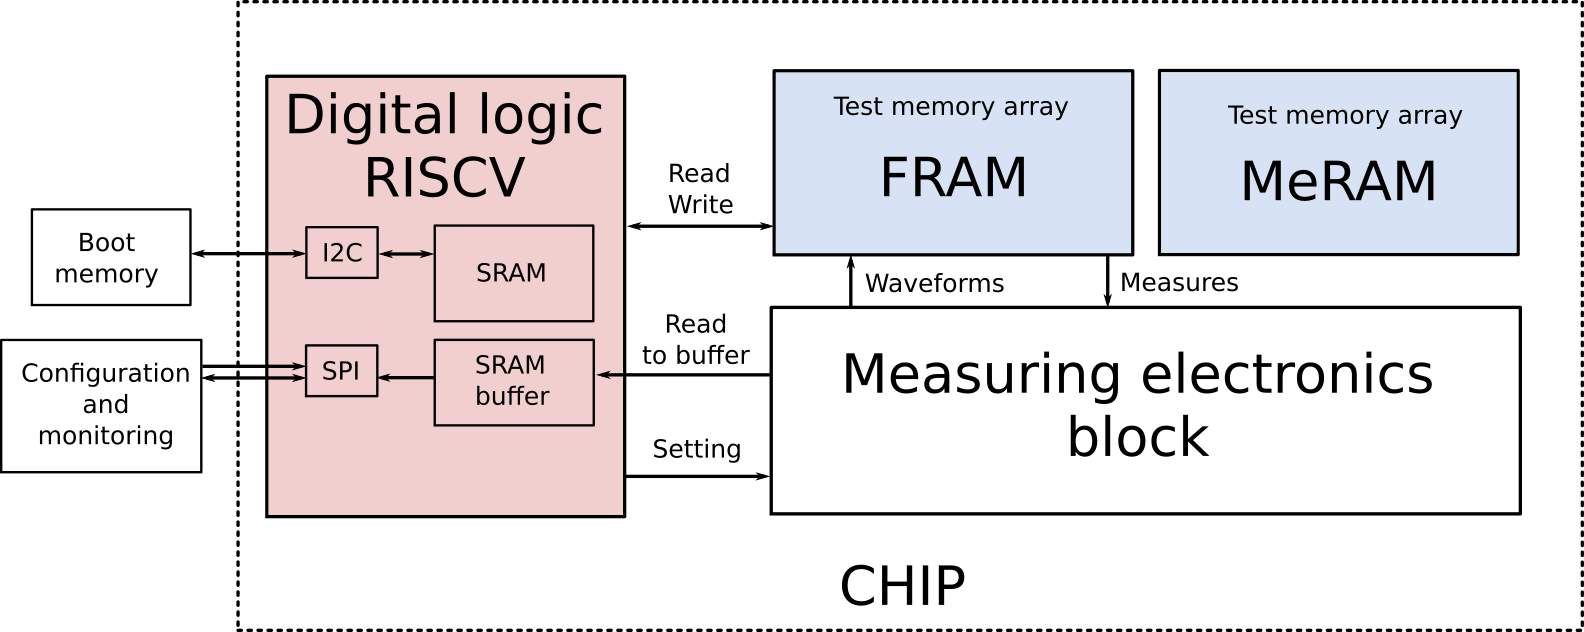
\includegraphics[width=\textwidth]{top.png}
\caption{Супер общая схема чипа}
\end{figure}

Примерное устройство чипа представлено на рисунке, и предполагает контроль/измерение нескольких ядер различной памяти,а также анализаторов отклика, с возможностью подключать их как к интересующим нас столбцам выбранного стека, так и к индивидуальной ячейки. Планируется покрыть спектр измерений ячеек, схожий с возможностями тестовой станции \link{https://www.keysight.com/ru/ru/assets/7018-01289/data-sheets/5989-2785.pdf}{B1500A} 

\paragraph{Ядро памяти (Test memory array)}\label{array}

Представляет собой почти обычное ядро памяти (для примера можно посмотреть ядро DRAM памяти (рис. \ref{DRAM})), только с конденсаторами интересующего нас оксида, а так же с драйвом (то есть подачей питания) для нижней обкладки. А так же необходимо продумать мультиплексер (переключатель) для подключения тестирующей аппаратуры к линиям стоков транзисторов и плейт лайнам.  

В принципе задача не требует создания супер компактного и продуманного ядра, поэтому можно сэкономить время не создавая различные пре-декодеры и системы сложной адресации.

\begin{figure}[h]
\centering
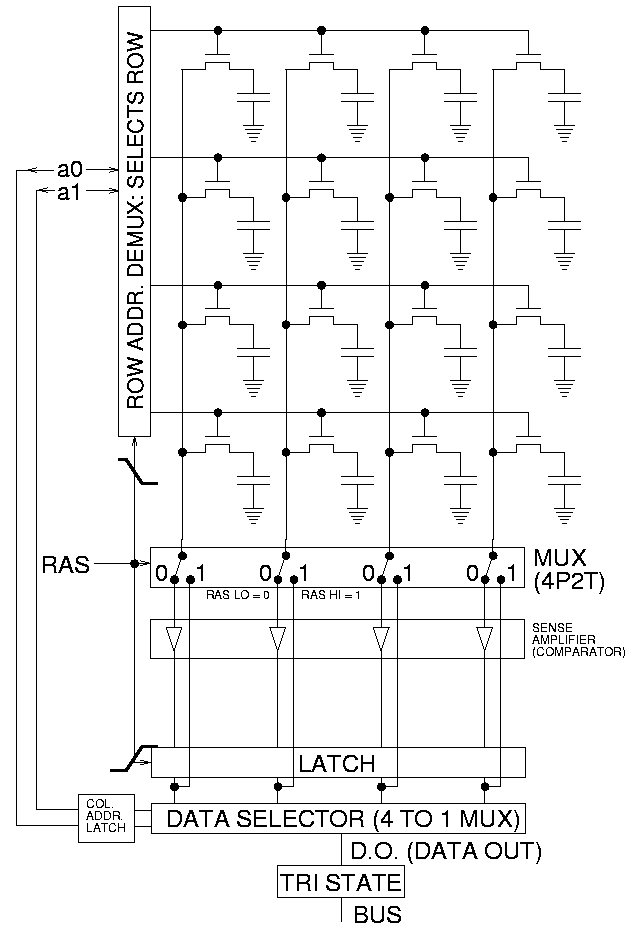
\includegraphics[width=0.5\textwidth]{Square_array_of_mosfet_cells_read.png}
\caption{Для понимания схема DRAM} \label{DRAM}
\end{figure}



\paragraph{Измерительная часть (Measuring electronics block)}

Самая сложная, аналоговая часть, способная подавать стимулы напряжения и тока в необходимые части исследуемого массива см. (\ref{array}). Предполагается реализовать возможности измерения схожие с  \underline{ \href{https://www.keysight.com/ru/ru/assets/7018-01289/data-sheets/5989-2785.pdf}{B1500A} }, однако лишенного минусов связанного с физическими зондами. 

Интересуют заданные измерения напряжений, ёмкостей и токов связанные в диапазоне не ниже 8 бит, для целой линии, или для одной ячейки.

Так же было бы желательно реализовать возможность записи относительно короткого промежутка измерения, но с хорошим битрейтом в буфер обмена контроллера (см. \ref{digital}), после чего уже передачу ее через интерфейс наружу.

\paragraph{ Контроллер чипа (Digital logic)} \label{digital}

Для управления измерениями прямо на чипе планируется реализовать микропроцессор поддерживающий набор инструкций RISCV (!), так же необходимая для него оперативная статическая память, необходимая память для буфера измерения, необходимая внутренняя периферия.

\subparagraph{Память} Количиство SRAM памяти очень жестко зависит от того сколько времени измерения мы хотим зафиксировать. К примеру современная SRAM на техпроцессе 90 nm имеет плотность 2 $mm^2/MB $ (\ref{pic:sram}), соответстветственно даже 2 Мб памяти уже будет большой роскошью. Для этого предлагается вынести часть оперативной SRAM так же на внешний чип. Рассчитывается записывать единоразово около 200 тысяч тиков измерения в буфер.

\begin{figure}[h]
\centering
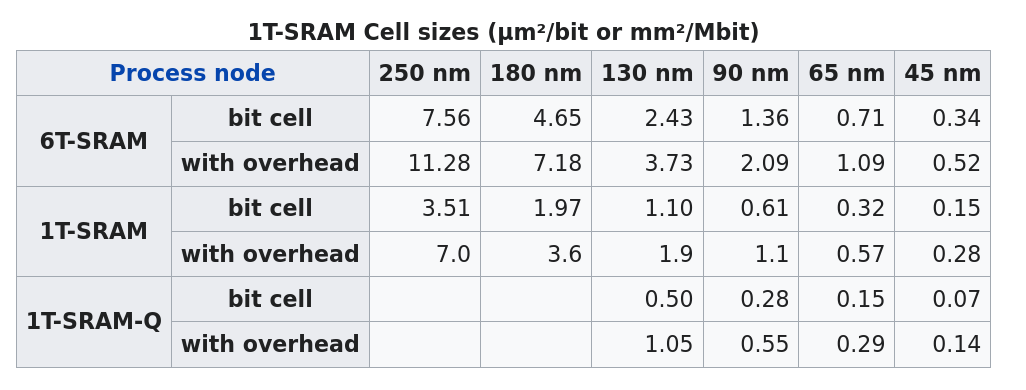
\includegraphics[width=0.8\textwidth]{sram.png}
\caption{ Плотность SRAM, источник Wikipedia}\label{pic:sram}
\end{figure}



\paragraph{ Переферия  (SPI , I2C)}

\subparagraph{SPI} Кажется разумным использовать SPI интерфейс для обмена данными с контроллером, а так же конфигурации всей системы использовать slave SPI, редактируя нужные блоки памяти контроллера тем самым производя необходимые настройки (подобно тому как это происходит при прошивке любого микроконтроллера).

\subparagraph{I2C}

Поскольку память на чипе энергозависимая, то необходимо реализовать некоторый загрузочный сектор, откуда можно подгрузить некую прошивку, и куда же ее можно сохранить. Для этого уместно использовать I2C интерфейс с подключенному к нему чипу  памяти вроде \link{https://www.fujitsu.com/downloads/MICRO/fsa/pdf/products/memory/fram/MB85RC64A-DS501-00019-2v0-E.pdf}{такого}.

\paragraph{ Тактирование (Clock)}
Для нормальной работы управляющей цифровой и измерительной аналоговой электроники требуется реализовать тактирование, причем если мы хотим проводить измерения с большим битрейтом (большой частотой), то нам нужен тактирующий сигнал большой частоты. Дима предложил два варианта (поправьте если я не так понял): Либо заводить сигнал нужной частоты в чип посредством \link{https://ru.wikipedia.org/wiki/LVDS}{LVDS}, либо по средством достройки частоты (ФАПЧ) увеличивать частоту обычного тактирующего резонатора. Так или иначе для измерений внутри должен где то быть клок порядка  ГГц и память способная быстро записать снятые измерения. По крайней мере таков план.


\section{Выполнение}





Предлагаю скоординировать коллектив, выполнение и постановку тактических задач в \underline {\href{todoist.com}{Todoist}}.

\subsection{Roadmap}

Предположительно придется уложиться вот в такие сроки (уточнить практическую возможность):


\begin{figure}[h]
\centering
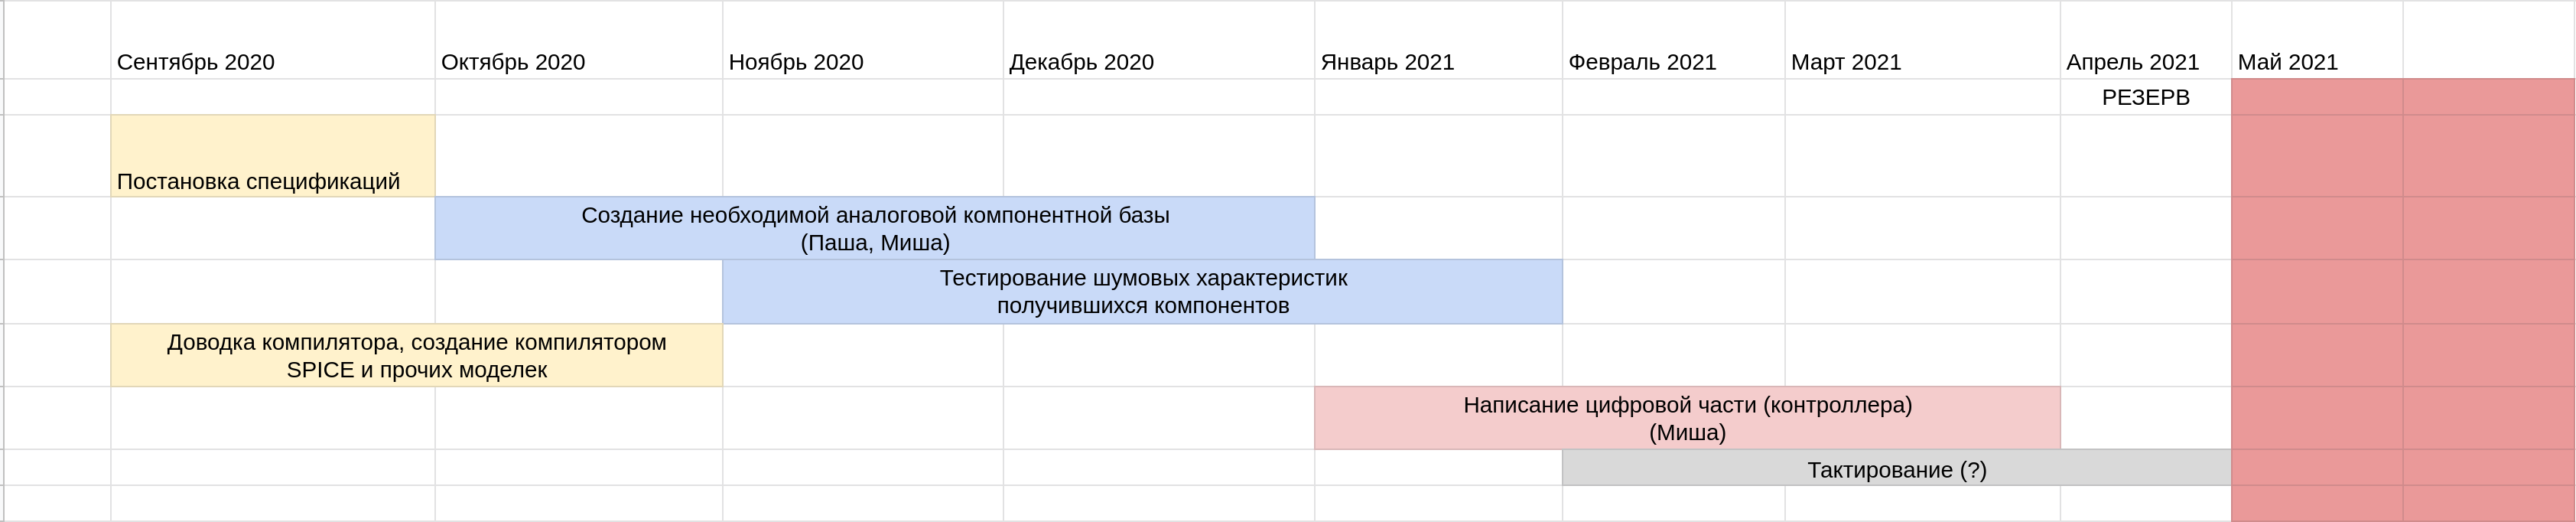
\includegraphics[width=1.1\textwidth]{roadmap.png}
\caption{ Черновик предлагаемой карты проекта}
\end{figure}

Актуальная ссылка на карту проекта:  \url {https://docs.google.com/spreadsheets/d/1iLgjOFxg0ekC7h_q5b4wdxDc1nRjKAJDCEXyratIL5U/edit?usp=sharing}



\subsection{Квалификации}

Ниже приведены необходимые  hard skills к выполнению задач, а так же люди подходящие под описание. Диму я исключил тут из всех категорий, но он есть во всех видимо.

\begin{itemize}
\item \textbf{Цифровая электроника} Разработка контроллера, имлементация verilog кода, настройка синтеза на кристалл. (Миша)
\item \textbf{Аналоговая электроника} Схемотехника, Симуляция, Создание Layout ячеек (Паша, Миша)
\item \textbf{Python programming} : создание компилятора для SPICE и физической репрезентации, возможно написание скриптов для отладки, тестирования, автоматизированной симуляции.(Паша, Миша)

\end{itemize}

Явно не хватает коллег для работы над аналоговой электроникой в виду огромного объема сопряженых с ней работ, а так же низкой возможностью автоматизации этого процесса.

\subsection{Имеющиеся Ассеты}

\begin{itemize}
\item Имеется недописанный \underline{\href{https://gitlab.com/mipt-ncs/nvram-gen}{компилятор ядра}}
\item В открытом доступе можно найти много verilog кода для RISCV архитектуры и перефирии.
\item SRAM компилятор для проекта от Микрона
\item У Димы есть готовый базовый чип памяти, но он плохо маштабируется. Можно использовать для референса  рабочего ядра. 


\end{itemize}

\end{document}